\documentclass[11pt,a4paper]{article}
\usepackage{shared-style}
\usepackage{graphicx}
\usepackage{float}
\usepackage{listings}
\usepackage[utf8]{inputenc}

\shorttitle{Final Statistics Project with R}
\shortauthors{Maltoni, de Mingo Arroyo, Peña}

\begin{document}

\papertitle{Final Statistics Project with R: Analysis of Various Techniques Applied to Heart Failure Data}
\paperauthors{Adam Maltoni, Ibón de Mingo Arroyo, Antonio Peña}
\paperdate{November 2024}

\begin{abstract}
In this work, a heart failure dataset is explored using data analysis and classification. Dimensionality reduction methods such as PCA and PLS are applied, along with clustering to group patients with similar characteristics. Finally, LDA is used to evaluate the classification capability of the variables, aiming to provide clinical knowledge about risk profiles and possible interventions. As a brief initial exploratory analysis, we show the distributions of the data (299 obs., 15 variables).
\end{abstract}

\tableofcontents
\newpage

\section{Introduction}
In this work, a heart failure dataset is explored using data analysis and classification. Dimensionality reduction methods such as PCA and PLS are applied, along with clustering to group patients with similar characteristics. Finally, LDA is used to evaluate the classification capability of the variables, aiming to provide clinical knowledge about risk profiles and possible interventions. As a brief initial exploratory analysis, we show the distributions of the data (299 obs., 15 variables).

\begin{figure}[H]
    \centering
    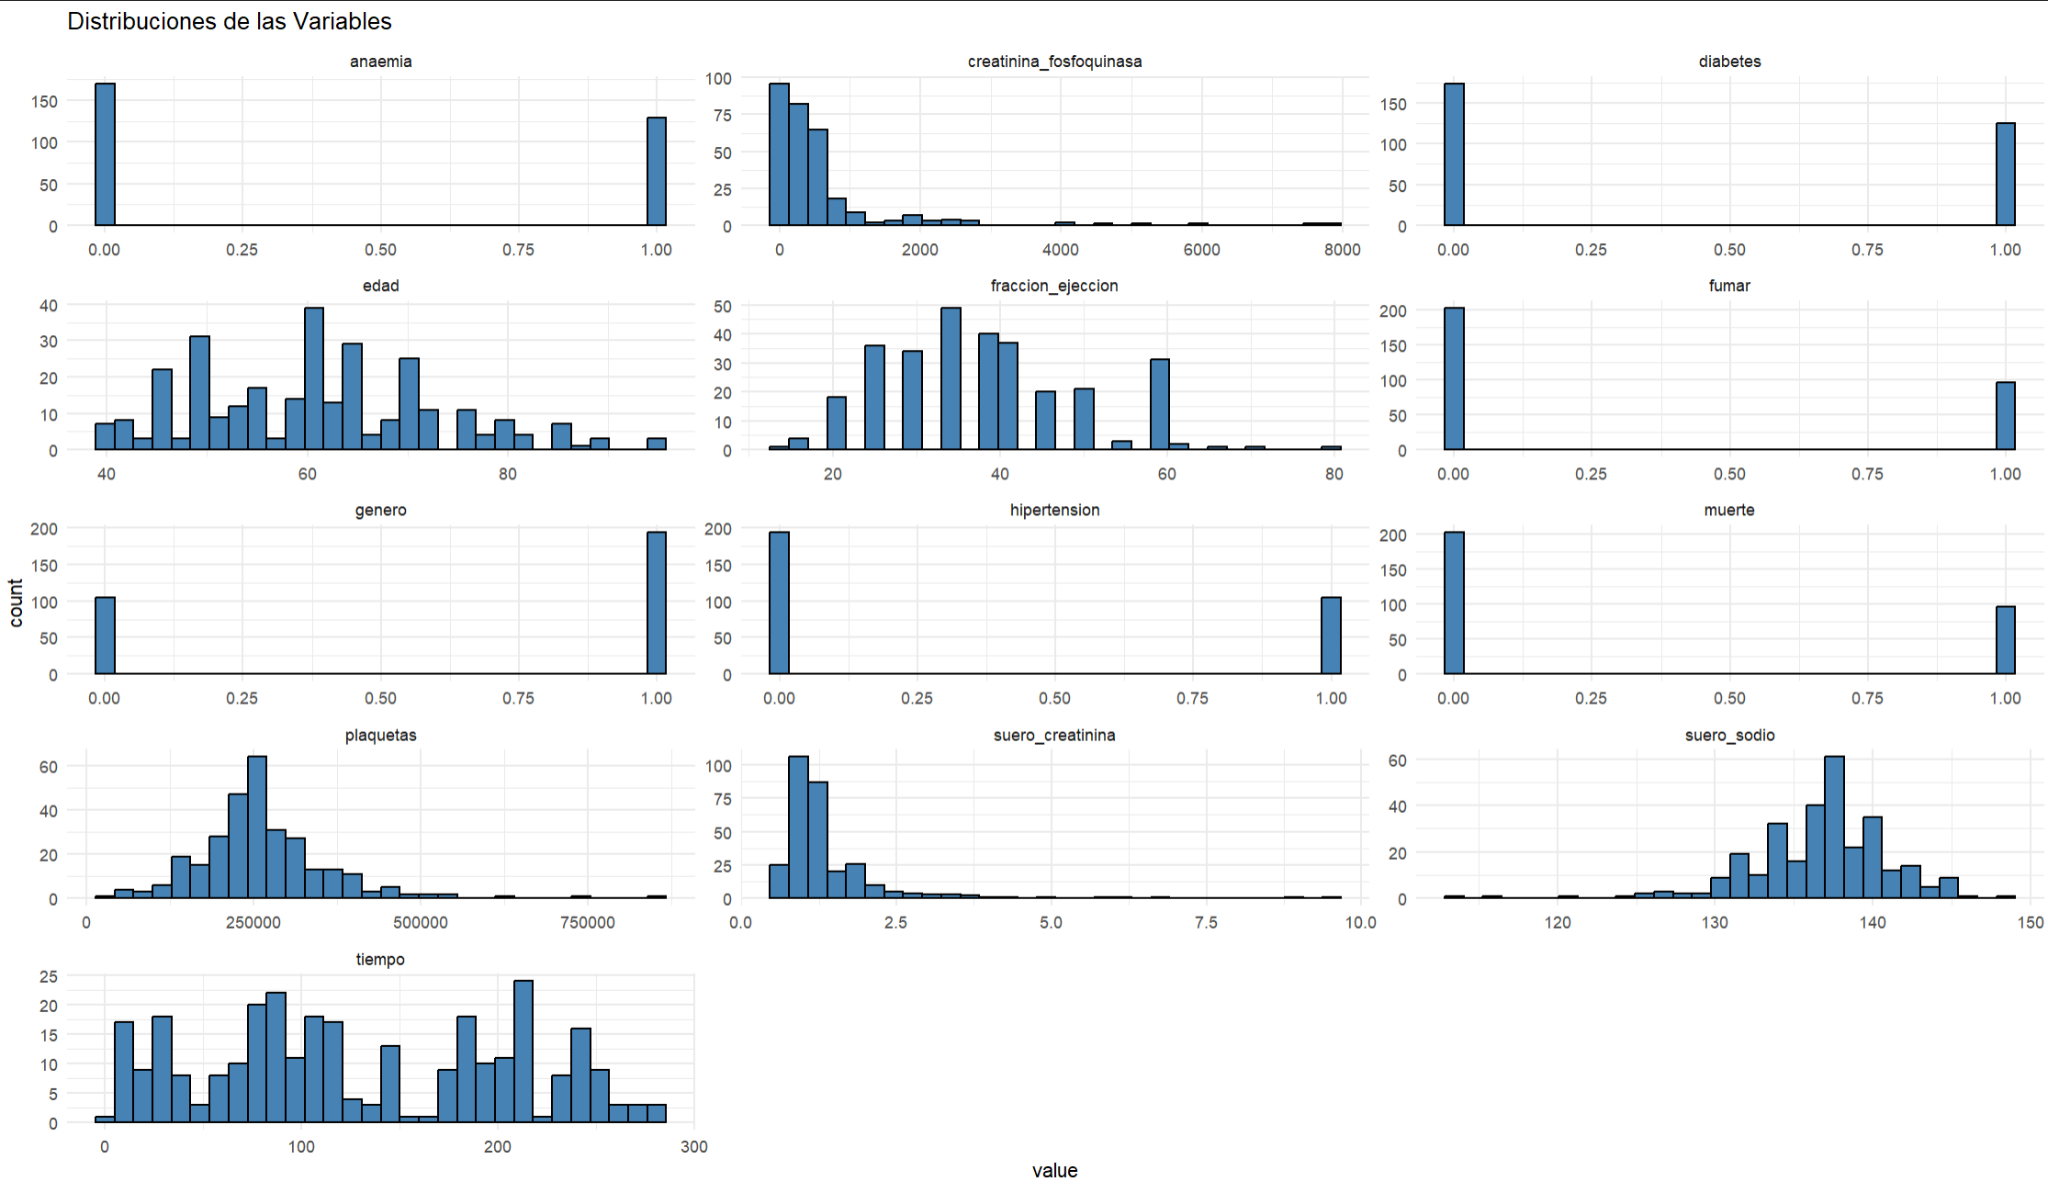
\includegraphics[width=0.8\textwidth]{img/page2_img1.png}
    \caption{Distributions of the data}
\end{figure}

\section{Principal Component Analysis (PCA)}
The goal of a PCA is always the same: (1) to identify underlying patterns in the continuous variables of the dataset; (2) to reduce dimensionality while preserving most of the variance; and (3) to visualize the data in a manageable dimensional space (for example, visualizing a dataset with 27 dimensions in 2 dimensions).

To do this, since PCA only works with numeric variables, we will choose only the continuous variables found in the dataset. Namely: age, phosphokinase\_creatinine, ejection\_fraction, platelets, serum\_creatinine, serum\_sodium, and time. After calculating the corresponding variables with the PCA method in R, we find the following:

\begin{figure}[H]
    \centering
    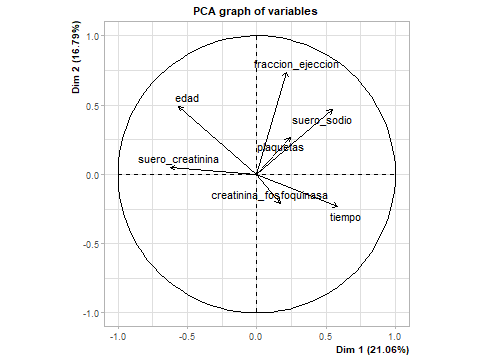
\includegraphics[width=0.8\textwidth]{img/page3_img1.png}
    \caption{PCA Output}
\end{figure}

Which means that the variables are not particularly correlated nor very well represented in the two-dimensional space. In fact, if we look closely, we can see that the variance explained by the first two components is only 37.85\%. If we look at the screeplot:

\begin{figure}[H]
    \centering
    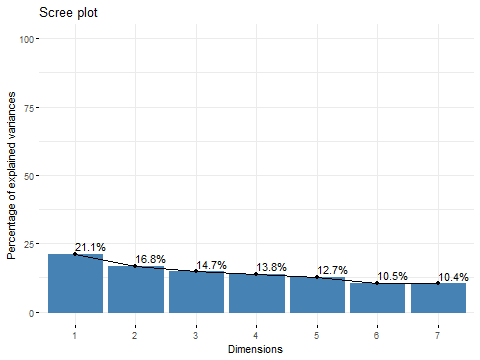
\includegraphics[width=0.8\textwidth]{img/page4_img1.png}
    \caption{Screeplot}
\end{figure}

Thus, we need up to 5 variables to accumulate almost 80\% of the variability (79.1\% with the first five variables). By considering 7 for the analysis, it is not very useful as a variable reduction tool. Most of the information (variance) is lost in the process unless we keep the vast majority of the variables. The low correlation of the variables among themselves is very clear when looking at the following graph:

\begin{figure}[H]
    \centering
    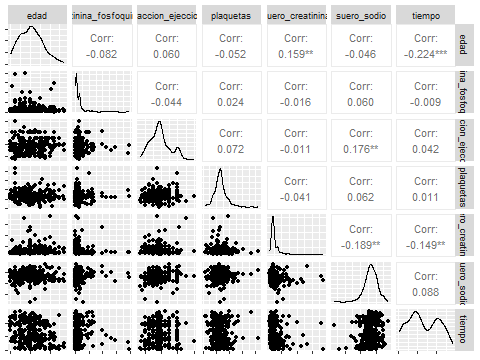
\includegraphics[width=0.8\textwidth]{img/page4_img2.png}
    \caption{Correlation plot}
\end{figure}

The strongest correlation occurs between age and time, with only -0.224. Finally, the representation of the data can be visualized using a biplot with some alpha (to avoid overloading certain areas with many points). Adding light colors, the result of the code is:

\begin{figure}[H]
    \centering
    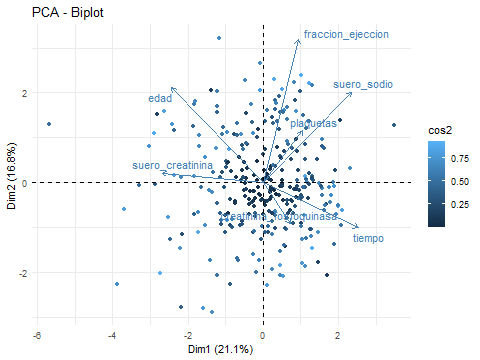
\includegraphics[width=0.8\textwidth]{img/page5_img1.png}
    \caption{Biplot}
\end{figure}

As can be easily seen, the points are distributed more or less randomly and uniformly throughout the graph, with a notable concentration of points around the center.

\section{Partial Least Squares (PLS)}
The fundamental usefulness of PLS is to achieve high predictive capability by discounting possible correlations between predictor variables. In this case, we want to predict whether a person will die or survive based on the data we have, which are provided in the dataset. After training the model in the manner seen in class, we see that with a few components we can drastically reduce the error to almost zero.

\begin{figure}[H]
    \centering
    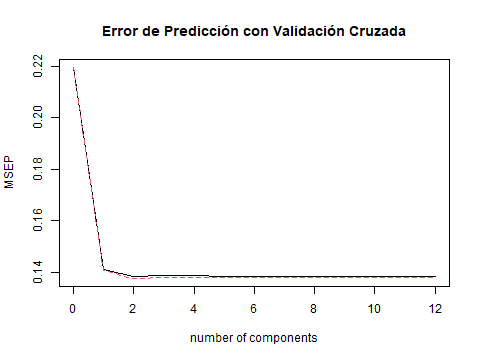
\includegraphics[width=0.8\textwidth]{img/page5_img2.png}
    \caption{PLS Error vs Components}
\end{figure}

The mean error starts low but is reduced to negligible levels in a jump by including more than one or two components. As a final result, having chosen only 2 components, we obtain a very high accuracy of 0.84280; with a confusion matrix characterized by being quite faithful to the real data.

\textbf{Confusion Matrix} \newline
Real \textbackslash{} Predicted \newline
False - True \newline
False: 185 - 18 \newline
True: 29 - 67

The analysis reveals that certain types of patients may have a higher risk of death than others depending on certain key variables. For example, elderly people with diabetes or who smoke. Young people in relatively good health have an extremely low risk of suffering cardiac arrest.

\section{Cluster Analysis}
Cluster analysis is an unsupervised learning technique that seeks to identify patterns in datasets by grouping similar observations into groups or "clusters". Each cluster contains elements that are more similar to each other than to elements in other clusters, according to some metric of similarity or distance.

In the context of medical data, as in our case, this technique is useful for identifying groups of patients with similar clinical characteristics. This can be key to designing personalized treatments, detecting common risk factors, and improving diagnostic accuracy. Therefore, we can intuit a priori that it is a suitable technique for our dataset.

For the analysis, continuous and integer variables representing health indicators have been selected, namely age, phosphokinase creatinine, ejection fraction, serum creatinine, serum sodium, and platelets. Categorical variables have not been selected because, generally, they are not included in common clustering techniques that we will use (especially K-means); usually, the obtained clusters are mixed with other categorical variables for interpretation at the end of the analysis, or other algorithms such as K-modes, K-means with Gower distance, or the KAMILA algorithm can be used.

Starting with the analysis itself, we first scale the data to ensure that we weigh all variables equally in the calculation of distances. Next, we try to determine the optimal number of clusters to use through two methods: the elbow method (WSS) and the silhouette index.

\begin{figure}[H]
    \centering
    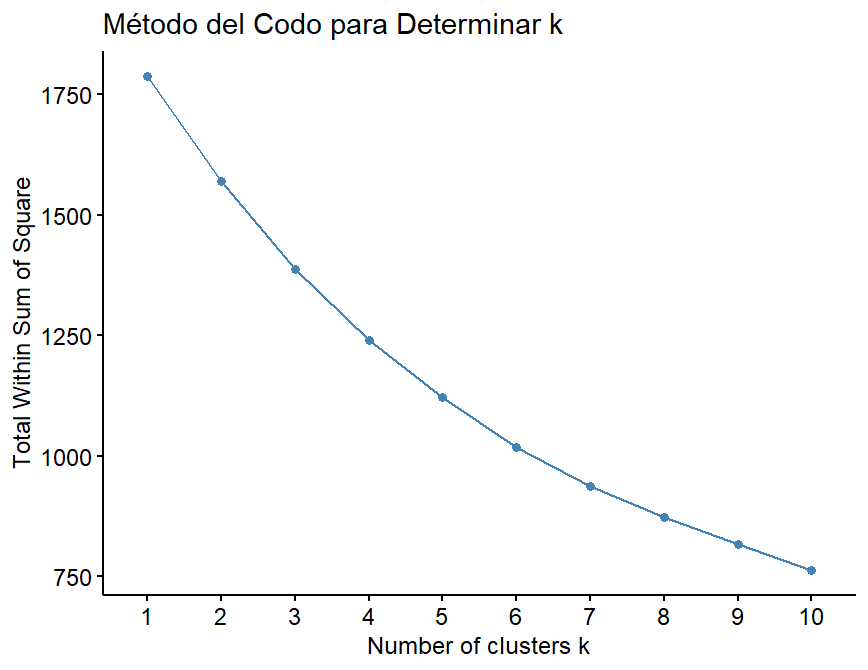
\includegraphics[width=0.8\textwidth]{img/page7_img1.png}
    \caption{Elbow method (WSS)}
\end{figure}

In this case, we would certainly choose to consider about 6 clusters as the optimal number, although there does not seem to be a clear inflection point in the curve defined by the WSS. On the other hand, according to the silhouette method, we obtain 4 groups as the optimal clustering, as we can see below by looking for the point with the highest silhouette index in the graph:

\begin{figure}[H]
    \centering
    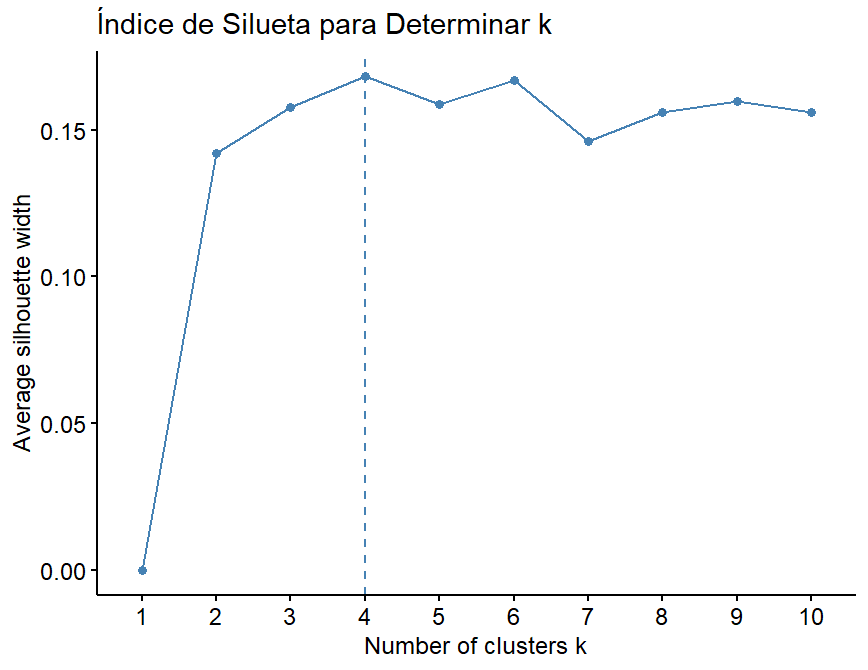
\includegraphics[width=0.8\textwidth]{img/page7_img2.png}
    \caption{Silhouette index}
\end{figure}

Furthermore, to finally confirm our hypotheses, a plot is produced where we test how the data would be grouped for each number of clusters between 1 and 10 according to a K-means algorithm.

\begin{figure}[H]
    \centering
    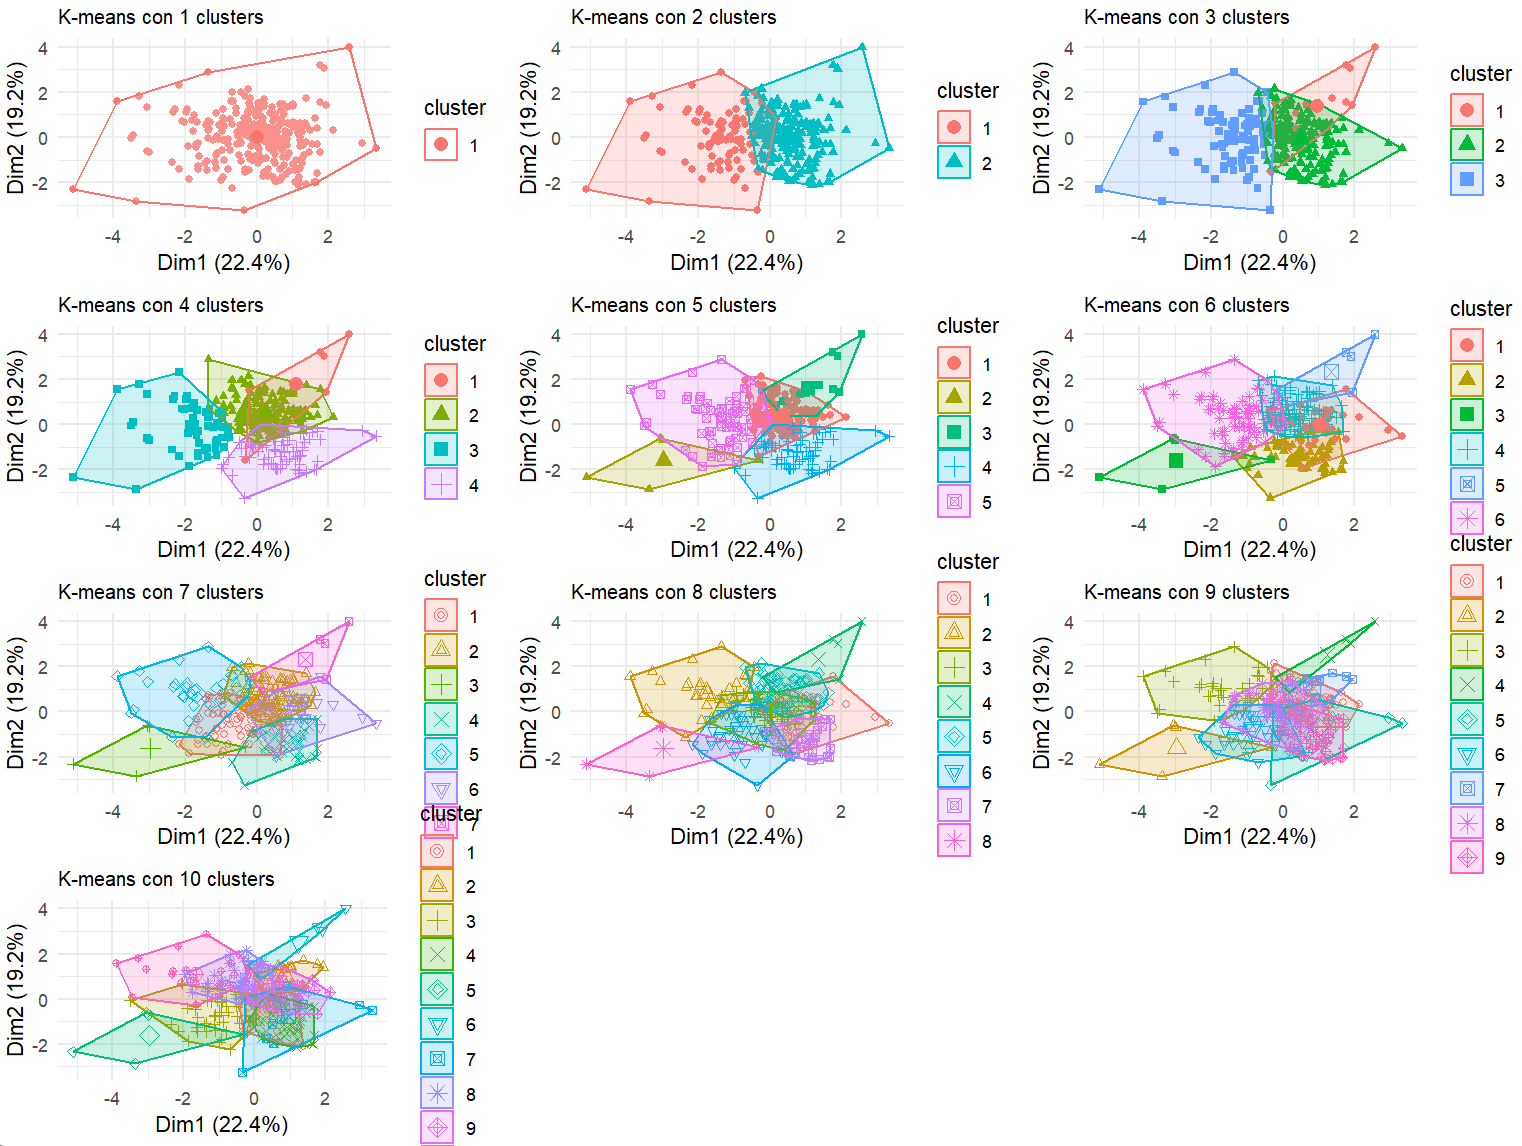
\includegraphics[width=0.8\textwidth]{img/page8_img1.png}
    \caption{K-means visualization 1}
\end{figure}

It can be seen that, based on the data, adding more clusters beyond 4 or 5 does not seem to have much effect at the separation level, although this may be due to the intrinsic structure of the representation (in 2D, they are being represented only as a function of the two attributes that explain the most variability, and, as mentioned in the PCA section, the variability of the dataset is very well distributed among variables, as we can see from the 22.4\% and 19.2\% of the axes). The data give the impression of being very centralized in this plot.

We analyze the obtained centroids to understand how each group differs clinically:

\textbf{Cluster 1:}
\begin{itemize}
    \item Mean age: 60
    \item Mean creatinine (serum): 1.854286
    \item Mean ejection fraction: 37.85714
    \item Mean platelets: 277388
    \item Mean serum sodium: 138.5714
    \item Cluster size: 7
\end{itemize}
Older patients with elevated creatinine, moderate cardiac function, and normal sodium levels, possibly with kidney damage.

\textbf{Cluster 2:}
\begin{itemize}
    \item Mean age: 55.77019
    \item Mean creatinine (serum): 1.119938
    \item Mean ejection fraction: 32.98137
    \item Mean platelets: 252995.8
    \item Mean serum sodium: 137.4534
    \item Cluster size: 161
\end{itemize}
Adults with reduced cardiac function and normal creatinine, probably in initial stages of heart failure.

\textbf{Cluster 3:}
\begin{itemize}
    \item Mean age: 69.78182
    \item Mean creatinine (serum): 2.516
    \item Mean ejection fraction: 34.18182
    \item Mean platelets: 226791
    \item Mean serum sodium: 131.5455
    \item Cluster size: 55
\end{itemize}
Elderly individuals with severe renal dysfunction, low sodium levels, and moderate to advanced heart failure.

\textbf{Cluster 4:}
\begin{itemize}
    \item Mean age: 65.17105
    \item Mean creatinine (serum): 1.119737
    \item Mean ejection fraction: 51.73684
    \item Mean platelets: 310480.3
    \item Mean serum sodium: 138.3684
    \item Cluster size: 76
\end{itemize}
Older patients with preserved cardiac function, normal creatinine, and good overall condition, possibly in recovery or with adequate control.

We see that if, for example, we put 10 clusters, the centroids would not vary much among themselves in attributes, and additionally, we would end up with several clusters with very few individuals.
(Note that the "diagnoses" have been issued with ChatGPT due to lack of medical knowledge by the students).

Now, we move on to hierarchical clustering, with three linkage strategies, considering the minimum, maximum, and average distance between points/clusters during their construction (single, complete, average). We obtain three dendrograms that we can compare:

\begin{figure}[H]
    \centering
    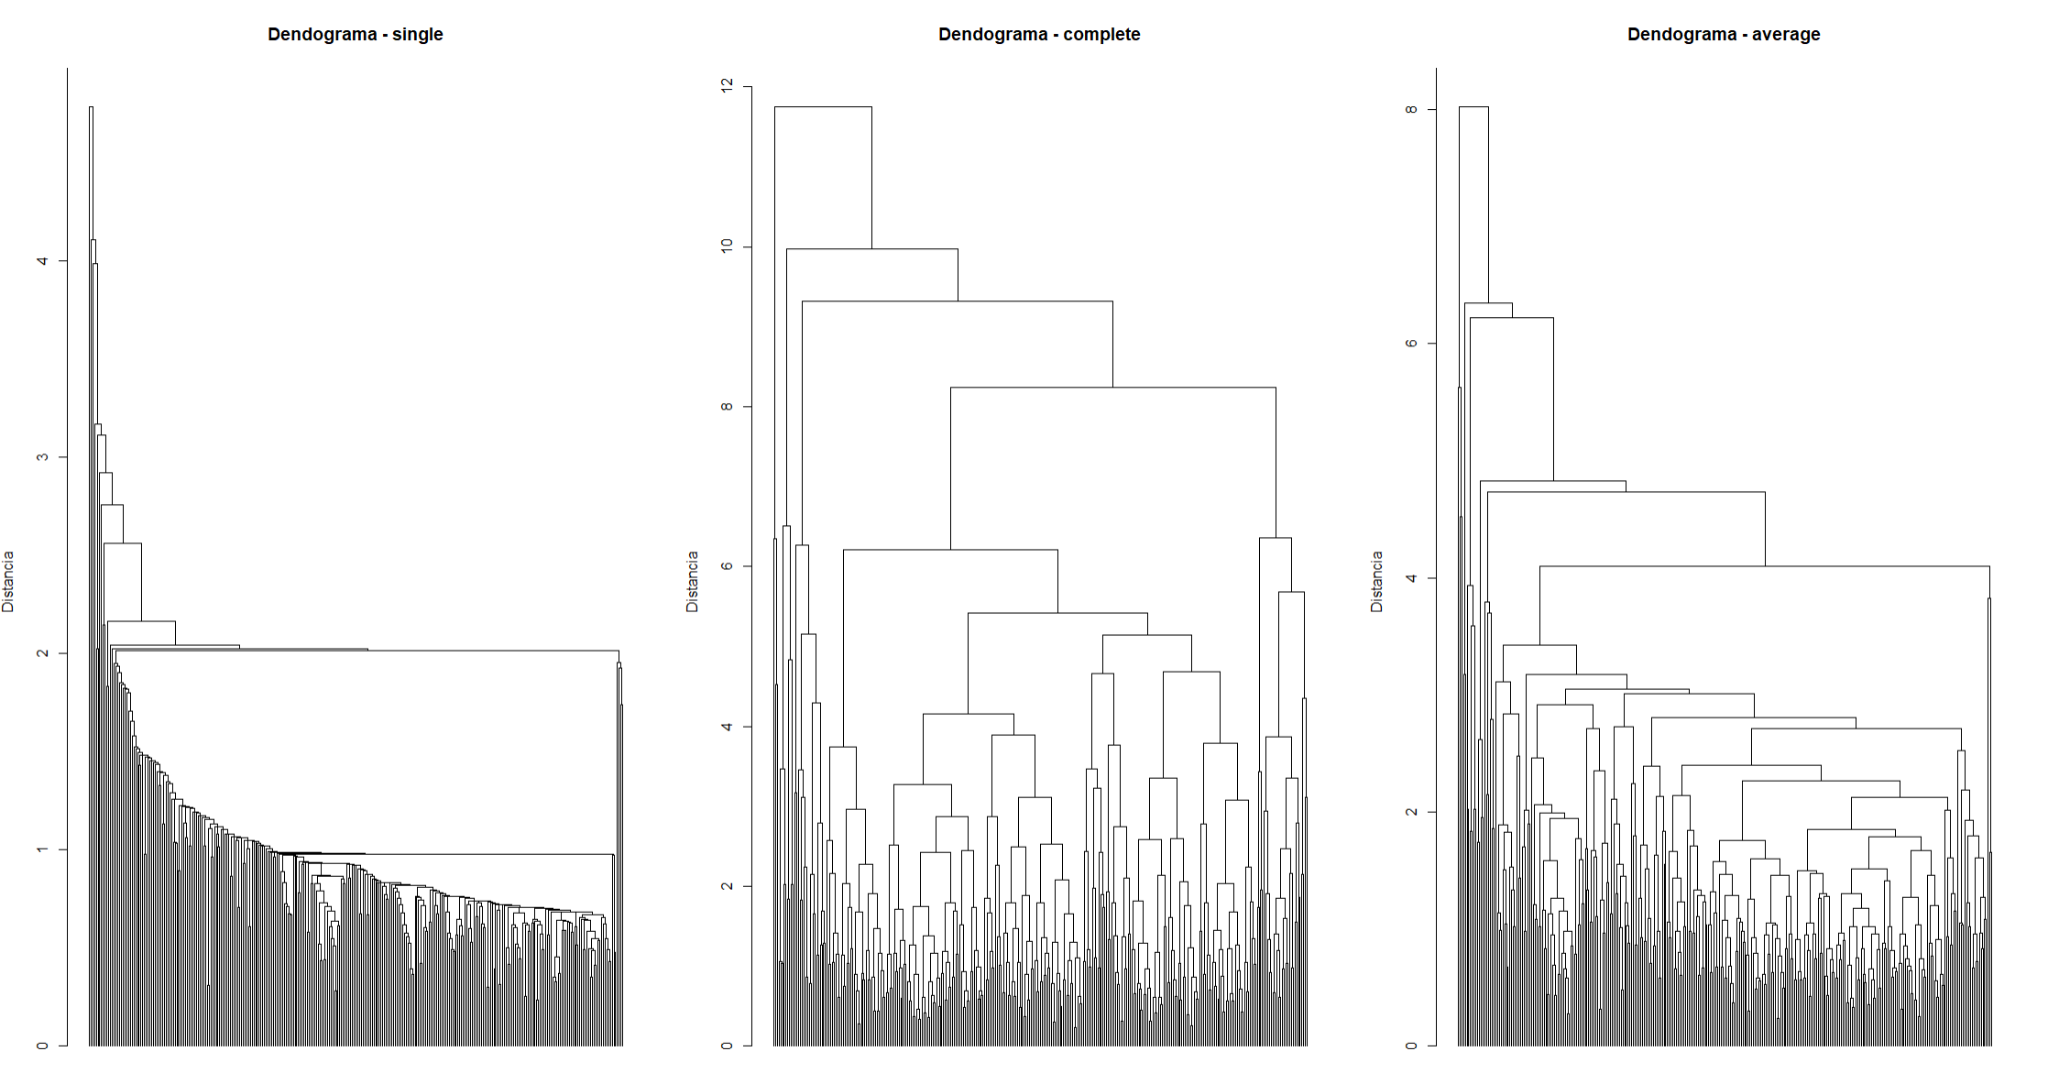
\includegraphics[width=0.8\textwidth]{img/page10_img1.png}
    \caption{Hierarchical clustering dendrograms}
\end{figure}

As we see in the dendrograms, the three distance metrics do not correspond particularly well when it comes to creating clusters, which suggests that entirely natural relationships among the data are not being found.

A posteriori, the results show that the cluster analysis has revealed groupings that make clinical and statistical sense, given that the groups differ in terms of age, serum creatinine, ejection fraction, etc. However, we see low concordance among the three hierarchical methods (change in distance) used, which may suggest that the data might not be perfectly separated into natural groups. Furthermore, it would be ideal to validate these results with clinical knowledge or correlations with medical outcomes, for example with the categorical variables left behind earlier such as smoking or death.

As an extracted conclusion, cluster analysis has provided useful segmentation of the dataset, highlighting significant clinical differences among the 4 considered groups, but there is room for improvement in the technique through the consideration of binary variables and because of the low concordance among the hierarchical methods, among themselves, and of these with the considered non-hierarchical K-means method, since at the end of the study we obtain a concordance of only 2.01\% between the hierarchical and non-hierarchical methods.

\section{Linear Discriminant Analysis (LDA)}
Linear Discriminant Analysis (LDA) is an analysis equivalent to linear regression in which categorical variables are classified. The goal is to identify linear relationships among continuous variables so that we can differentiate between predefined groups. Furthermore, an attempt is made to define a decision rule that allows for the correct classification of a new object, whose group membership is unknown, by assigning it to the most appropriate group. To carry it out, it is important that a series of assumptions are met:

The target variable must be categorical, which in our dataset is fulfilled since it is binary. And the variables chosen to carry out the analysis must be continuous, therefore the following variables are selected: age, phosphokinase creatinine, ejection fraction, serum creatinine, serum sodium, and platelets. It is also necessary that for each group of the binary variable, two or more observations are available, which is fulfilled in our dataset. Also, when performing the analysis, the number of discriminating variables must be less than the number of observations minus two. That is, if we have p discriminating variables and n individuals, then $p < (n - 2)$.

Before performing LDA, it must be verified that no discriminating variable is a linear combination of the other discriminating variables. To do this, we show the covariance matrix.

\begin{figure}[H]
    \centering
    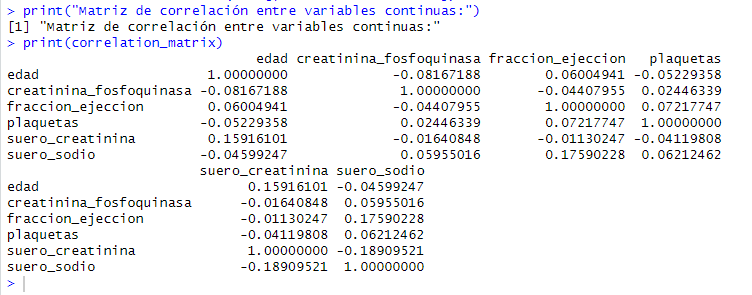
\includegraphics[width=0.8\textwidth]{img/page12_img1.png}
    \caption{Covariance matrix}
\end{figure}

In the matrix, no high correlation is observed (the highest is close to 0.2 which is adequate) so we will continue checking the rest of the assumptions.

LDA assumes that continuous variables must follow a normal distribution. To do this, we visualize it with histograms and will perform a check with code using the Kolmogorov-Smirnov test studied in previous courses.

\begin{figure}[H]
    \centering
    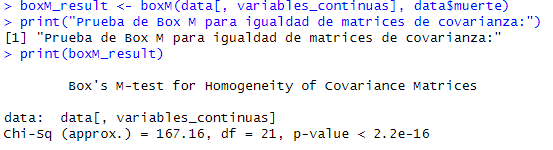
\includegraphics[width=0.8\textwidth]{img/page13_img1.png}
    \caption{Histograms}
\end{figure}

In the histograms, it seems that generally the variables do not follow a normal distribution, and after performing the test, we observe that most p-values are less than 0.05, so a normal distribution is not followed. The only one with a p-value greater than 0.05 is age, which has a p-value of 0.1.
We will continue checking the assumptions.

Finally, the last assumption is that the covariance matrices within each group must be approximately equal. To do this, we will use boxM() which will measure whether they are equal or not.

The null hypothesis of this test is that the covariance matrices are equal among the different groups. When performing the test, we see that the p-value is much less than 0.05, so we reject the null hypothesis that the covariance matrices are equal among the groups.

Despite the fact that the assumptions are not met and therefore the model may be biased or inefficient, we will perform the analysis to study the results. Before running the model, we standardize all variables.

Observing the discriminants, we see that the ejection fraction variable has a coefficient of -0.62, which indicates that lower values in this variable are more likely to belong to the group that died. On the other hand, the serum creatinine variable with a coefficient of 0.57 indicates that the higher the value of this variable, the more likely the patient is to die. A higher age also contributes significantly to the probability of death. These three variables are the most important for differentiating the group to which each patient belongs. However, variables such as platelets (0.025) and diabetes (0.12) seem to have less influence on the model.

After performing the model, we make predictions with which we obtain the following results:

\begin{figure}[H]
    \centering
    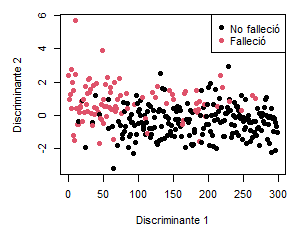
\includegraphics[width=0.8\textwidth]{img/page14_img1.png}
    \caption{LDA Predictions}
\end{figure}

Visually it seems that the model has been able to differentiate both classes with some precision, but to be sure, we will evaluate the accuracy of the model which gives us: 0.7558528

Although the model achieves an accuracy of 75\%, the fact that the assumptions are not met makes the results not completely reliable. It is possible that the model is biased or that the generalization capability with other data is not good.

\section{Conclusion}
In this study, techniques such as PCA, PLS, clustering, and LDA have been combined to analyze heart failure data. PCA helped to reduce dimensionality, PLS highlighted key variables for predictions, clustering identified patient profiles, and LDA evaluated their classification. Together, these techniques offer a more comprehensive view of the dataset, aimed at improving clinical analysis and the prediction and prevention of possible deaths.

\section{Bibliography}
1. Tools and software
[1] R Core Team. "The R Project for Statistical Computing." https://www.r-project.org/.
[2] RStudio. "RStudio IDE Documentation." https://posit.co/products/open-source/rstudio/.

2. Information about the techniques used
[3] Brownlee, J. "A Gentle Introduction to Principal Component Analysis (PCA)." Machine Learning Mastery. https://machinelearningmastery.com/introduction-to-principal-component-analysis/.
[4] Statology. "Partial Least Squares (PLS) Regression in R." https://www.statology.org/pls-regression-in-r/.
[5] Wikipedia. "Cluster Analysis." https://en.wikipedia.org/wiki/Cluster\_analysis.
[6] Tutorials Point. "Linear Discriminant Analysis." https://www.tutorialspoint.com/linear\_discriminant\_analysis.htm.

3. Learning resources and tutorials
[7] Towards Data Science. "A Guide to PCA in R with Examples." https://towardsdatascience.com/a-guide-to-principal-component-analysis-in-r-with-examples-654d856633be.
[8] GeeksforGeeks. "Clustering in R." https://www.geeksforgeeks.org/clustering-in-r/.

\end{document}
